\documentclass{aas}
\setsansfont[Extension = .ttf, BoldFont = *-Bold]{Euclid}
\usepackage{xurl}
\Urlmuskip=0mu plus 2mu
\setlength{\emergencystretch}{2em}
\hypersetup{pdftitle={整身运动规划中的几何表征与约束转换综述},pdfauthor={},pdfsubject={AI辅助论述初稿，未投稿}}
\begin{document}
\cntitle{整身运动规划中的几何表征与约束转换综述}
\cnauthor{}
\cnabstract{整身运动规划需要显式处理机器人形状与姿态，并协调几何保真度、优化可处理性和安全保证的适用范围。本文围绕几何表征如何转换为规划约束，以及这些转换如何影响可行运动、目标代价和保证语义，综述可微碰撞查询、凸自由区域与连续时间避障的代表性研究。通过统一描述几何模型、约束语义、数值求解过程与验证假设，区分最终判定中的保守几何与仅用于筛选的几何、连续轨迹表示与连续时间约束满足、区域统计性质与单条轨迹风险等不同问题。利用二次Bézier曲线的解析案例说明：充分包含条件可能拒绝安全曲线，而精确分段可使同一曲线通过认证。进一步讨论学习几何、不确定性以及规划与执行之间的接口，形成有条件的方法选型和评价建议。本文采用定向文献检索与相关技术段落核验，不将其表述为穷尽式系统综述或新的实验基准。}
\cnkeyword{整身运动规划; 几何表征; 碰撞检测; 凸自由区域; 连续时间约束; 安全保证}
\entitle{Geometric Representations and Constraint Transcription in Whole-Body Motion Planning: A Review}
\enauthor{}
\enabstract{Whole-body motion planning requires explicit treatment of robot geometry and orientation, while balancing geometric fidelity, optimization tractability, and the scope of safety guarantees. This review examines how geometric representations are transcribed into planning constraints and how these transformations affect feasible motions, objective functions, and the interpretation of guarantees. Representative studies on differentiable collision queries, convex free-space regions, and continuous-time collision handling are compared using a common description of geometric models, constraint semantics, numerical solution procedures, and validation assumptions. Three distinctions are emphasized: conservative geometry used for final acceptance differs from geometry used only for screening; a continuously parameterized trajectory does not by itself establish continuous-time constraint satisfaction; and a region-level statistical statement does not directly imply a trajectory-level collision probability. An analytic Bézier example illustrates how a sufficient containment condition can reject a safe curve and accept the same curve after exact subdivision. The review further discusses learned geometry, uncertainty, and the planning--execution interface, and derives conditional guidance for method selection and evaluation. The synthesis is based on a targeted literature search and verification of relevant technical passages, rather than an exhaustive systematic review or a new experimental benchmark.}
\enkeyword{whole-body motion planning; geometric representation; collision detection; convex free-space regions; continuous-time constraints; safety guarantees}
\cnaddress{}
\enaddress{}
\doi{}
\cstr{}
\makeatletter
\let\caddress\@empty
\let\aas@enaddress\@empty
\let\aas@doi\@empty
\let\aas@cstr\@empty
\makeatother
\maketitle
\pagestyle{plain}\thispagestyle{plain}
\noindent\textbf{审阅版 v0.4（2026-11-11）}\quad AI辅助形成的论述初稿，尚未投稿。已核验题录、相关技术段落与解析图；最近综述全文对照及独立编码尚未完成。\par\medskip
机器人在狭窄通道、受限操作空间和高速运动场景中的可行性，常由整个占据体积而非单一参考点决定。把机器人简化为质点并膨胀障碍，在形状固定、仅考虑平移等适用条件下可以有效降低问题复杂度；当姿态改变了通行能力，或关节运动使各部件扫过不同区域时，固定膨胀模型就可能损失关键运动。如何将完整几何信息转化为能够高效处理的规划约束，因而成为整身运动规划的重要问题。尺度优化碰撞评估、机器人本体坐标系距离场及自由区域构造分别从几何查询、信息复用与空间结构化角度回应这一问题。\cite{R01}\cite{R07}\cite{R02}

运动规划综述已有较为广泛的积累。面向多旋翼的综述将自由空间提取、轨迹参数化与控制范式联系起来，几何导航综述覆盖几何理论及算法应用，风险校准综述则明确讨论不确定性、可认证安全与资源约束。\cite{S02}\cite{S06}\cite{S07} 制造机器人安全综述进一步以优化和可行性联系感知与运动规划，协同变道综述强调执行权限、名义优化及端到端保证的区别。\cite{S09}\cite{S10} 中文综述也已从多机器人任务与运动规划的协同关系组织技术进展。\cite{J01} 因此，“兼顾安全与实时性”或“从全流程讨论规划”已经不足以构成新的综述视角。

仍有必要细化的比较问题是：同样被称为精确、可微或连续无碰撞的技术，其结论究竟约束了哪个对象。单状态碰撞查询精确，不意味着离散路点之间没有碰撞；区域内碰撞体积分数较小，不意味着某条特定轨迹风险较低；轨迹在参数空间中缩短，也不意味着物理空间中的路径同步缩短。已有研究分别揭示了这些问题，但跨方法选型时，若只保留算法类别、运行时间和成功率，就会掩盖其适用前提。\cite{R15}\cite{R21}\cite{R30}

本文以“表征---约束---求解---验证”的接口为分析单位，重点完成三项综合：第一，区分几何近似作为最终约束、优化代理或分级筛选时的不同作用；第二，对可微碰撞查询、凸自由区域和连续时间约束采用一致的保证对象与失败原因编码；第三，将这些条件转化为可追溯的方法选择与评价建议。这里的集合关系和解析例子用于解释已有机制，不作为新定理或新规划算法。对于最近综述尚未完成全文对照的部分，本文不主张该组织方式具有首创性。

\section{研究范围与证据组织}
本文将整身无碰撞规划界定为显式约束机器人占据集合的运动规划。配置q(t)包含必要的位置、姿态或关节变量；B(q(t))是机器人在工作空间中的占据集合，O(t)是障碍集合。研究以移动刚体的姿态相关几何为起点，引入机械臂文献讨论配置空间、运动学耦合和自碰撞。本文不把“整身”限定为人形机器人的接触力分配，也不尝试覆盖操作技能、任务语义与接触动力学的全部问题。

比较围绕四个问题展开：表征是否保留参考几何下的可行运动；有限约束如何关联连续运动；求解输出在何种容差和运动模型下成立；几何结论如何连接感知与跟踪误差。文献按实际承担的功能交叉归类，同一方法可以同时属于距离查询、轨迹优化和执行接口，而不被强制分配到互斥的算法名单中。

本稿检索截至2026年11月11日，采用题名与关键词检索、原始文献引用追踪及近邻综述反向对照。关键词围绕whole-body collision、differentiable collision、convex free space、configuration-space certification、swept volume与continuous collision组合展开，并补充中文碰撞检测、整身运动规划和轨迹优化。来源以出版社、会议论文集、作者机构与固定版本预印本为主。当前证据集属于目的性选择的代表文献集，不据此估计整个领域的文献占比或增长率。

纳入对象须明确涉及几何查询、区域构造、轨迹约束或保证边界；只有算法名称相近、但没有对应几何机制的工作，不作为技术论证依据。预印本与正式版本按方法族关联，保留实际读取版本，避免将版本更新计成独立方法。对于2024年预印本、2026年期刊发表的区域构造工作，技术判断与发表状态分别记录。\cite{R15} 正式发表的2026年中文机械臂规划研究也纳入背景比较，但摘要层证据不被提升为定理或性能复验。\cite{R31}

证据核验区分题录、摘要及引言、相关技术段落、全文编码并复核四个层级。核心比较优先使用已核对的模型、定理条件、算法步骤与局限段落；只有摘要证据的研究用于标识分支，不承担优越性结论。本文没有运行新的规划实验，也没有汇总不同硬件和任务下的性能数字形成排行榜。检索尚未达到穷尽式覆盖，核心文献的完整双人编码和最近综述的全文差异核验，仍是投稿前须完成的工作。

\section{几何约束转换的共同描述}
为避免把任务定义变化误认为算法改进，先固定规划时域、起终条件、动力学及非碰撞约束，令$\Gamma$表示满足这些共同条件的连续运动集合。参考无碰撞集合F由机器人和障碍的参考模型定义；它是比较基准，不等同于具有未知感知误差的真实世界。下式约定接触即不满足严格分离要求；若具体方法允许边界接触，必须同步改变判定语义。

\begin{equation}
\begin{aligned}\mathcal F=\{q\in\Gamma:\ &B(q(t))\cap O(t)=\varnothing,\\&\forall t\in[0,T]\}.\end{aligned}
\end{equation}
表征层用代理几何或自由区域定义可接受运动集合$F_R$。编码层再用有限变量、分段表示和约束定义可重构轨迹集合$F_E$。若代理占据集合外包参考几何，且代理确实用于最终硬判定，则$F_R$包含于F；若有限约束充分保证表征层的连续无碰撞，则$F_E$包含于$F_R$。两个包含关系均有条件：内近似、软罚项、未经覆盖证明的时间采样，可能使编码接受参考模型中的碰撞轨迹。图1总结这种条件传递。

\begin{equation}
\mathcal F_E\subseteq\mathcal F_R\subseteq\mathcal F.
\end{equation}
数值求解与几何集合也应分开。令$S_B$表示预算B内实际生成的候选轨迹，V表示验证器接受的轨迹集合，最终输出来自$S_B$与V的交集。一般不能预设$S_B$包含于$F_E$，因为提前终止、软约束、有限精度或实现误差都可能留下违反约束的候选。只有求解过程已满足相应可行性条件时，才能把该包含关系用于论证。

\begin{equation}
\mathcal A_B=\mathcal S_B\cap\mathcal V.
\end{equation}
这一区分避免两种常见误推。其一，外包几何若仅用于快速证明分离，而所有不能确认分离的状态都转交精细检查，并不必然缩小最终可行集；分级碰撞检查中的筛选与最终约束作用不同。VAMP展示了向量化和分层查询可以服务于已有规划框架。\cite{R29} 其二，固定候选集上的末端过滤不能补回缺失轨迹，但验证若参与后续搜索，就可能改变候选集。Lazy PRM通过碰撞检查更新图并重新搜索，正是已有的反馈式验证机制。\cite{R28}

即使可行集在坐标映射下保持一致，目标函数也可能发生变化。对于光滑坐标变换q=$\phi$(z)，选定参考坐标中的欧氏弧长包含映射的雅可比，而直接累加参数坐标中的欧氏距离会采用不同度量。对于混合位置、姿态和关节坐标，还必须先约定量纲与度量，不能把下式直接当成任意配置的物理路程。关于GCS参数化空间失真的研究说明，约束可行性与目标代价需要分别比较。\cite{R21} 因此，本文用“排除安全运动”“接受不安全运动”“求解未找到”“目标度量改变”描述不同失败来源，而不把所有现象归结为几何精度。

\begin{equation}
L(q)=\int_0^T\!\sqrt{\dot z^{\mathsf T}J_\phi(z)^{\mathsf T}J_\phi(z)\dot z}\,{\rm d}t.
\end{equation}
\begin{figure*}[t]
\centering
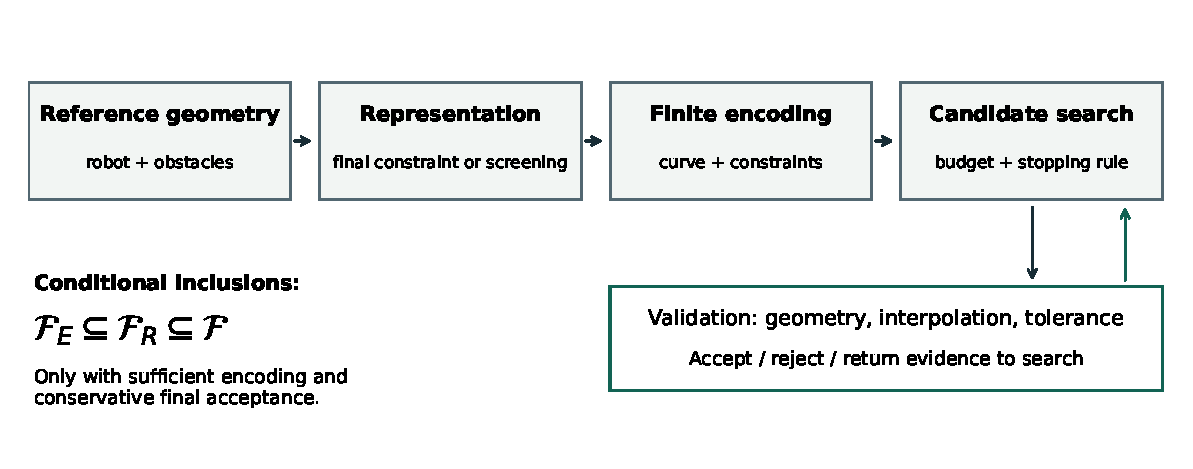
\includegraphics[width=.96\textwidth]{figures/constraint-chain.pdf}
\bicaption{几何表征至验证的条件传递。包含关系依赖最终判定语义；验证可反馈搜索。自绘概念图，不是实验结果。}{Conditional interfaces from geometry to validation; validation can feed back into search.}
\end{figure*}
\section{可微碰撞查询：数值含义与优化用途}
碰撞查询为规划器提供几何值与导数，但“可微”描述的是局部计算性质，“精确”描述的是相对于给定模型的数值或判定关系，两者都不直接等价于规划问题容易求解。对于非凸机器人，分解方式、部件数量及部件间最小值聚合还会引入额外的复杂度与非光滑性。对方法进行比较时，应先记录输入几何和输出量，再讨论导数及求解代价。表1给出代表性路线的接口区别。

基于优化的碰撞避免（Optimization-Based Collision Avoidance，OBCA）利用凸优化对偶将适用凸集之间的避碰关系转写为便于优化处理的约束，为位置、姿态与物体尺寸联合进入规划提供了基础。\cite{R04} 这种等价转换以原几何模型及对偶成立条件为前提，并不保证外层非线性轨迹优化获得全局最优解。把局部几何子问题的凸性直接迁移到整个规划问题，是不同层级之间的混淆。

尺度优化路线考察两个凸体按规定中心缩放到首次接触所需的尺度。线性尺度评估针对多面体模型建立线性规划，并提供适于优化的梯度或次梯度信息。\cite{R01} DCOL以可组合凸基元及凸优化形式计算类似尺度量，并通过优化问题的敏感性获得导数。\cite{R05} 这些量具有明确的几何判定含义，但通常是无量纲尺度，而非米制欧氏距离。将尺度余量直接当成固定米制安全距离，会因对象尺寸、缩放中心及姿态而改变含义。

对接触切换和尖角导致的非光滑性，可以采用随机平滑或正则化。随机平滑路线提供用于梯度计算的平滑机制；2026年的解析接触导数研究进一步通过相应正则化模型处理接触运动学的求导条件。\cite{R06}\cite{R16} 这里应区分被平滑的几何量、被求导的替代问题以及原始实体的碰撞关系。隐函数求导依赖解和相关系统的正则性，不能仅凭方法可返回一个梯度，就推断所有配置处都具有唯一、稳定且几何保真的导数。

机器人本体坐标系欧氏符号距离场（Robo-centric Euclidean Signed Distance Field，RC-ESDF）将几何信息预计算在机器人坐标系中，使障碍点通过位姿变换进入查询，适合讨论不规则形状与在线复用。\cite{R07} 该路线把计算负担从反复构造环境场转向局部查询，但准确性仍依赖场的构造、采样分辨率、插值方式和障碍输入。任意形状的表达能力，不等同于有限离散数据对任意环境都给出精确碰撞判断。

因此，局部查询评价至少应报告模型相对于参考几何的误差、查询量的单位、接触附近的导数行为，以及这些因素对下游轨迹可行性的作用。仅比较微秒级调用耗时，无法判断完整规划过程是否更快；单次查询较慢的方法也可能通过更有用的导数减少迭代。后者必须由同一任务、初值和计算预算下的证据支持，不能从导数形式直接推导。

\begin{table*}[t]
\centering
\bicaption{代表性几何查询的接口与结论边界}{Interfaces and limits of representative geometric queries}
\small\setlength{\tabcolsep}{3pt}
\begin{tabular}{>{\raggedright\arraybackslash}p{0.225\textwidth}>{\raggedright\arraybackslash}p{0.225\textwidth}>{\raggedright\arraybackslash}p{0.225\textwidth}>{\raggedright\arraybackslash}p{0.225\textwidth}}
\toprule
路线与文献 & 查询或约束对象 & 可支持的判断 & 不能直接推出\\
\midrule
OBCA \cite{R04} & 适用凸集的对偶避碰约束 & 在模型与对偶条件下的等价关系 & 外层非线性规划全局最优\\
尺度LP / DCOL \cite{R01}\cite{R05} & 首次接触尺度及敏感性 & 对应缩放模型的碰撞判定 & 尺度量等于米制距离；处处光滑\\
随机平滑 / iDCOL \cite{R06}\cite{R16} & 平滑或正则化问题的导数 & 满足正则条件的局部导数信息 & 原几何未改变；无条件保守外包\\
RC-ESDF \cite{R07} & 本体坐标系距离场查询 & 给定场与障碍输入下的几何评价 & 离散输入已完整覆盖全部障碍\\
\bottomrule
\end{tabular}
\end{table*}
\section{凸自由区域：区域证书与下游规划}
凸自由区域将复杂障碍关系压缩为区域包含约束，使轨迹优化可以复用几何结构。迭代区域膨胀方法（Iterative Regional Inflation by Semidefinite programming，IRIS）交替构造分离超平面和内切椭球，为局部自由区域膨胀提供了基础。\cite{R10} 快速迭代区域膨胀（Fast Iterative Region Inflation，FIRI）强调给定种子集合的包含，并针对二维、三维的几何子问题组织高效计算。\cite{R02} 这两类方法首先回答“什么区域可以被安全使用”，而区域之间如何连接、能否满足动力学，以及如何选择运动，仍属于后续规划问题。

区域质量的指标必须与结论保持对应。FIRI的可行性叙述包括种子集合包含及区域内部无障碍，单调性结论针对内切椭球体积；这不等价于多面体体积逐轮增大，也不等价于找到全局最大自由区域。\cite{R02} 若原条件是障碍与区域内部不交，闭区域边界仍须结合接触约定理解。直接让机器人或曲线贴着边界运行，需要额外核对余量，而不是把“内部无障碍”改写为严格正间隔。

工作空间与配置空间的区域用途也不同。中心轨迹位于工作空间区域，不足以保证机器人所有点均在区域内；姿态、尺寸及外包关系需要另外进入约束。配置空间区域则把关节运动学和自碰撞纳入自由配置的描述。C-IRIS在有理参数化的配置空间中构建可认证多面体，使用多项式证书支持区域无碰撞判断。\cite{R11} 相应存在性结论依赖模型和多项式阶数等条件，不意味着给定固定阶数与有限时间一定能认证任意期望区域。

IRIS-NP2与IRIS-ZO利用采样和优化改善高维区域构造，并给出与区域碰撞体积分数相关的终止测试。\cite{R15} 若测试在指定均匀采样测度及独立性等条件下控制错误接受概率，其对象仍是区域的体积统计性质。规划器可能主动选择穿过狭小碰撞子集的路径，因此不能把区域级概率结论直接解释为每条路径的碰撞概率上界。改变参数坐标还会改变体积和均匀分布，比较时必须记录所采用的测度。

图凸集（Graphs of Convex Sets，GCS）方法将连续区域选择与区域内路径优化联系起来。\cite{R12} 它的保证需要同时限定给定区域覆盖、允许的曲线族、约束凸性以及松弛和舍入步骤；这些前提不能自动扩展到一般刚体或机械臂的非线性动力学。更大的单个区域可能方便优化，但覆盖遗漏关键通道、区域重叠不足或参数空间代价失真，都可能降低最终任务表现。\cite{R21} 表2据此区分区域几何证书与规划层结论。

\begin{table*}[t]
\centering
\bicaption{自由区域方法的保证对象与规划接口}{Guarantee objects and planning interfaces of free-space region methods}
\small\setlength{\tabcolsep}{3pt}
\begin{tabular}{>{\raggedright\arraybackslash}p{0.225\textwidth}>{\raggedright\arraybackslash}p{0.225\textwidth}>{\raggedright\arraybackslash}p{0.225\textwidth}>{\raggedright\arraybackslash}p{0.225\textwidth}}
\toprule
方法族 & 保证对象 & 关键条件或限制 & 下游需补充\\
\midrule
IRIS / FIRI \cite{R10}\cite{R02} & 给定几何下的凸区域；内切椭球等代理量 & 分离模型、种子条件、内部与边界区别 & 整身包含、覆盖连通、动力学与余量\\
C-IRIS \cite{R11} & 参数化配置空间内的区域证书 & 有理模型、多项式证书及可用阶数 & 坐标映射、区域覆盖与轨迹可执行性\\
NP2 / ZO \cite{R15} & 区域碰撞体积分数相关统计检验 & 采样测度、独立性、容许比例与错误接受参数 & 候选轨迹的独立验证\\
GCS \cite{R12}\cite{R21} & 既定区域图与可表示轨迹族中的优化 & 凸性、松弛/舍入、物理与参数坐标度量 & 覆盖外路径、一般非线性动力学\\
\bottomrule
\end{tabular}
\end{table*}
\section{连续时间约束：参数化、转录与运动模型}
连续参数化与连续时间可行性是两个不同属性。多项式可以在任意时刻求值，但如果避碰约束只在有限路点上施加，采样之间仍可能出现碰撞。TrajOpt已经将步间扫掠几何纳入序列凸优化中的碰撞处理，说明连续碰撞考虑本身并非新的研究空白。\cite{R08} 当前应比较的是不同方法采用什么插值运动、几何近似和数值条件，而非仅按是否出现“连续”一词划分安全等级。

有限采样若要推出整个区间的分离，需要可检验的覆盖条件。例如，令d(t)为满足已知Lipschitz界L的参考几何间隔；采样覆盖区间两端，最大相邻间隔为h，则任意时刻距某个采样点不超过h/2。由此得到下式。它给出充分条件，而不是仅靠提高采样频率就能获得的无条件保证。L必须对应实际几何运动和所用间隔函数；对任意缩放值直接套用米制距离的变化率并不成立。

\begin{equation}
\min_{t\in[0,T]}d(t)\geq\min_i d(t_i)-\tfrac12 Lh.
\end{equation}
凸包性质提供另一种有限编码。在适用的参数空间中，Bézier控制点都位于同一已验证凸区域，可以充分保证整条曲线位于该区域。图凸集轨迹构造采用这一类结构。\cite{R12} 其保守性可以由图2的解析案例直接看出：取矩形P=[-0.1,1.1]$\times$[0,1]，控制点依次为(0,0.2)、(0.5,-0.1)、(1,0.2)。曲线满足x=t、y=0.05+0.6(t-0.5)$^2$，最小纵坐标为0.05，因而始终位于矩形中；但中间控制点在矩形外，单段控制点包含条件不能认证它。

在t=0.5处用精确细分将该曲线表示为两段后，控制点分别为(0,0.2)、(0.25,0.05)、(0.5,0.05)及(0.5,0.05)、(0.75,0.05)、(1,0.2)，全部位于P内。同一条运动因表示方式改变而通过充分条件，说明被排除的可能是证书可表达性，而不是几何可行性。这个案例是标准凸包性质的解释性推导，不构成实验结果，也不说明所有安全曲线都能在给定分段预算下被认证。

紧凑多项式表示与连续约束转录之间同样需要划清界限。MINCO通过结构化参数化支持几何受限的多旋翼轨迹优化。\cite{R13} 时间均匀MINCO竞速工作利用边界结构处理穿门等式，同时将其他连续时间不等式转录为采样罚项。\cite{R03} 因而同一规划器内部可以并存精确处理的边界条件和近似处理的一般避障条件，不能给整篇论文统一贴上“所有约束严格满足”的标签。

扫掠体符号距离场直接把连续运动的占据几何纳入距离查询，为复杂形状提供另一条路线。\cite{R09} 但连续几何表达与外层优化成功仍是不同问题。该研究的局限讨论承认非凸优化下并非总能实现完全连续避障，并讨论三维计算和动态障碍方面的限制。将其标题中的连续无碰撞解释为任意初值和预算下都能返回安全解，会超出原文支持范围。

验证器还必须采用与输出一致的运动模型。cuRobo的v2技术报告明确以相邻路点之间球心直线运动进行相关检查，并指出转动关节连杆的实际运动并非如此。\cite{R30} 因此，线性球心轨迹的检查结论不能直接迁移到任意关节插值。FCL早期报告对实体包含与表面相交的讨论也提醒我们，网格精细程度不能替代碰撞语义的明确规定。\cite{R27} 这些是所读历史版本的边界，不用于断言当前软件仍有同样限制。

\begin{figure*}[t]
\centering
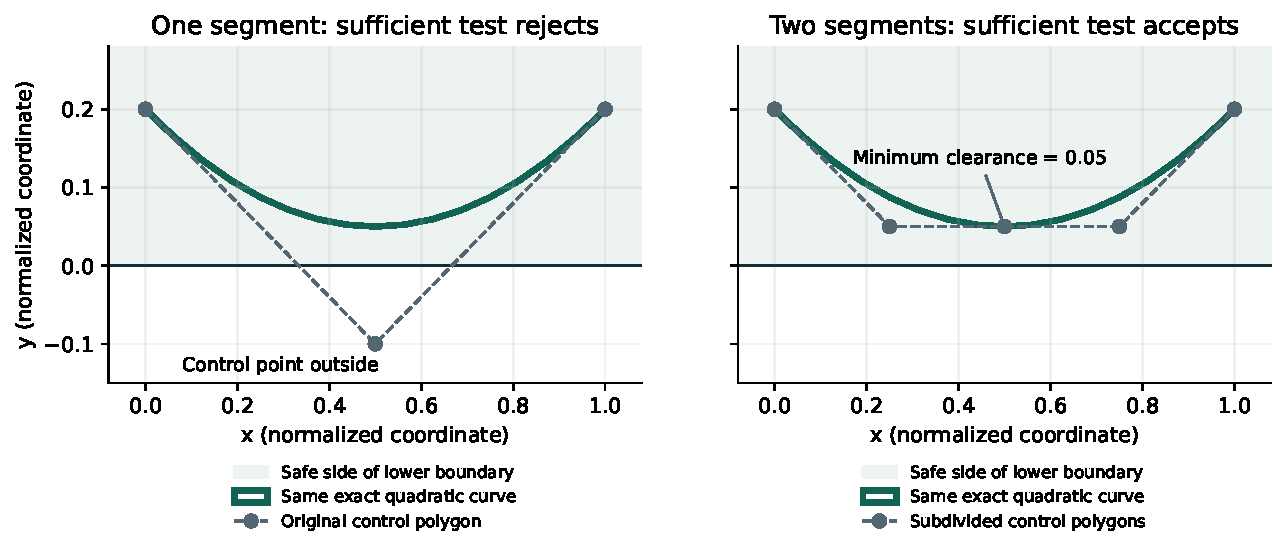
\includegraphics[width=.96\textwidth]{figures/bezier-certificate.pdf}
\bicaption{安全曲线被单段控制点包含条件拒绝，精确分为两段后通过。坐标为无量纲解析量；自绘，非仿真或实机数据。}{A safe curve rejected by a one-segment containment test and certified after exact subdivision.}
\end{figure*}
\section{学习、不确定性与执行接口}
即使参考模型下的连续轨迹无碰撞，真实执行仍受到感知、定位、障碍预测和跟踪误差影响。可靠的接口应说明误差加在机器人占据集合、障碍集合、状态分布还是控制可达集合上。Funnel Libraries和FaSTrack已经通过反馈可达集合与跟踪误差界联系规划和执行。\cite{R24}\cite{R25} 因此，把规划与控制联合考虑不能被当作尚未被研究的新空白；更有用的问题是某种几何表示是否能一致地接收这些误差界。

一个基础接口是几何扰动余量。若机器人和障碍的真实占据集合分别与名义集合具有已知Hausdorff距离界$\epsilon$\_B和$\epsilon$\_O，则两集合间最短距离的变化不超过两误差界之和。只有当这些界在所讨论时间区间内同时成立，并与同一坐标和几何定义一致时，名义间隔大于$\epsilon$\_B+$\epsilon$\_O才构成真实分离的充分条件。该条件不能凭经验指定一个安全系数来代替，也不处理未被集合界覆盖的障碍出现或感知漏检。

\begin{equation}
\begin{aligned}&\operatorname{dist}(B_{\rm real},O_{\rm real})\\&\quad\geq\operatorname{dist}(B_{\rm nom},O_{\rm nom})-\epsilon_B-\epsilon_O.\end{aligned}
\end{equation}
学习式几何查询用离线训练降低在线计算代价，同时引入拟合误差、分布变化和校准问题。RDF把可达运动的几何信息与神经隐式安全约束联系起来。\cite{R14} 比较这类方法时，应分别记录训练对象是单状态距离还是运动扫掠距离、输出是否有误差界、测试分布如何与部署分布关联，以及下游使用硬约束还是罚项。平均拟合误差低，并不能排除安全临界配置中的局部大误差。

2026年的随机神经扫掠体预印本将预测不确定性引入轨迹优化，但其推导包含高斯建模及一阶传播近似，不同规划形式也采用不同的约束处理。\cite{R17} 这些条件限定了概率语句的含义；不能把单点、单次查询或近似分布下的置信表述直接称为整段任务的零碰撞保证。U-OBCA进一步展示了几何对偶与分布鲁棒机会约束结合的方向。\cite{R18} 对后者，本文当前只采用摘要层证据识别研究分支，不比较其未经逐项核验的定理强度或数值优越性。

完整评价还应覆盖在线链路：环境数据更新、几何查询或区域生成、轨迹求解、输出验证，以及指令生效前的等待。硬件并行度、批量大小、离线预计算、重规划周期和超时处理共同决定部署意义。学习方法的推理加速与几何方法的查询加速，应在同一链路边界内比较，否则容易把局部计算优势误写成系统实时性结论。

\section{方法选型与证据可比性}
综合比较的目的不是给不同保证排出一个无条件优劣顺序，而是识别瓶颈与可采取的动作。表3从具体失败现象出发，区分几何表征、有限编码、数值搜索和执行误差；这些现象需要不同证据才能诊断。例如，优化器没有返回路径，既可能是区域覆盖确实封闭了通道，也可能是初值或预算不足，不能仅从一次失败判断任务不可行。

面向狭窄通道，应先检查最终约束是否使用过度外包的几何，再检查区域是否保留姿态相关通道。若当前粗几何只用于安全分离筛选，则细化它主要改变检查成本，未必改变最终可行性。面向高速或薄障碍场景，应首先检查时间覆盖与插值运动，而不是仅增加空间网格精度。面向高维机械臂，应同时记录自碰撞、关节坐标映射及区域认证成本。

比较实验若被用于后续版本，必须统一机器人实体、障碍输入、起终条件、动力学限制和验证规则。原始作者在各自条件下报告的成功率仍可被引用，但需要保留分母、失败定义、计算预算和硬件背景。没有同一验证模型和场景集的数据，不宜画成速度---安全二维优劣图。对于安全方法，输出数、通过验证数、超时数和拒绝数应分别呈现，避免通过不返回困难任务来获得表面上的零碰撞。

验证规则应在比较前固定，并接受自身审查：说明网格是否闭合、接触如何判定、时间如何覆盖、容差如何设置以及运动如何插值。验证器的接受并不是超越模型的真实安全证明。若条件只支持名义几何下的判定，应在结果中保留该限定。对于统计性声明，还须区分区域采样概率、查询误差概率与整条轨迹风险，不能把它们合并成同一“安全率”。

本文据此提出最低报告字段：参考几何与近似方向、模块用途、轨迹重构方式、约束实施位置、求解停止条件、验证运动模型、误差与概率假设、总计算边界。该字段集是本文的分析组织工具，其用途在于使不同研究可以被逐项核对；其充分性与跨场景实用性仍需更多文献编码和后续独立评价。

\begin{table*}[t]
\centering
\bicaption{按失败来源组织的条件化选型建议}{Conditional method selection organized by failure source}
\small\setlength{\tabcolsep}{3pt}
\begin{tabular}{>{\raggedright\arraybackslash}p{0.225\textwidth}>{\raggedright\arraybackslash}p{0.225\textwidth}>{\raggedright\arraybackslash}p{0.225\textwidth}>{\raggedright\arraybackslash}p{0.225\textwidth}}
\toprule
现象 & 需区分的原因 & 针对性动作 & 必要核验\\
\midrule
关键通道被封闭 & 最终外包几何或区域覆盖过保守 & 细化形状、姿态接口或区域连接 & 同一参考模型下存在可行运动的证据\\
安全曲线未通过约束 & 充分条件或分段表示受限 & 精确细分、改用适当证书 & 曲线本身保持不变；预算增加被计入\\
路点安全、步间碰撞 & 时间覆盖或插值模型不足 & 覆盖证书、扫掠检查或运动模型对齐 & 所用变化率界、旋转及关节运动\\
模型可行、求解失败 & 局部搜索、初值或数值预算 & 改进初始化、搜索与终止策略 & 约束残差和失败状态；不改写为不可行\\
名义安全、执行越界 & 感知、预测或跟踪误差未覆盖 & 误差集合与规划---控制接口 & 界的来源、有效时域及失效处理\\
\bottomrule
\end{tabular}
\end{table*}
\section{研究展望}
第一，几何保真度与导数质量需要放在同一任务中评价。精确尖角几何、平滑替代和学习近似各有计算优势，也可能产生不同的接触行为。值得推进的是同时报告原几何误差、导数稳定性和最终验证表现，并分析误差是否集中在决定通行能力的少数配置上。DCOL、随机平滑与解析接触导数已经构成这一方向的技术基础，未来贡献应超出单纯再次提出“几何可微”。\cite{R05}\cite{R06}\cite{R16}

第二，自由区域的质量评价应更直接服务于下游任务。体积、面数、种子包含和区域重叠具有不同作用；任务所需的运动方向、姿态通道和动力学可达性，可能比单一体积更能解释规划成败。研究可以在固定参考几何和轨迹目标的条件下比较这些因素，而不能通过更换目标或放松约束制造区域质量提升。FIRI、高维IRIS和参数度量修正提供了可衔接的研究基础。\cite{R02}\cite{R15}\cite{R21}

第三，连续时间证书与实时计算之间需要可中断、可解释的接口。局部细分、分级检查和验证反馈可能使计算集中于临界运动区间，但任何提前终止都应明确返回的是已认证结果、未经认证候选还是失败状态。Lazy PRM和向量化采样规划已表明，验证与搜索的组织方式本身能够改变计算成本。\cite{R28}\cite{R29} 新机制应说明它保持哪些判定语义，而不只报告平均加速。

第四，学习几何和不确定性推断需要与可审计的约束层结合。近期研究已将神经扫掠体、分布假设和机会约束接入规划。\cite{R17}\cite{R18} 后续应关注训练分布之外的误差、连续时间风险累计、校准失效及回退机制，而非把网络输出的置信度直接解释为物理安全概率。对于缺乏可靠误差界的场景，先明确结论的统计范围，往往比扩大形式上的保证措辞更有研究价值。

最后，可复查的比较资料应成为综述产出的组成部分。文献版本、模型假设、关键页码和表格编码可以公开为不含版权全文的证据清单，使读者能够追溯每一项技术归类。本文的后续修订需要进一步补齐最近综述全文对照、经典原始研究覆盖和独立复核；若这些对照显示相同组织已被充分完成，则应收缩问题范围，而不是依靠增加文献数量维持新颖性表述。

\section{结论}
本文围绕整身运动规划中的几何表征与约束转换，比较可微碰撞查询、凸自由区域和连续时间避障的代表性路线。共同分析表明，保证的含义由几何模型、模块用途、有限编码、求解条件与验证运动共同限定：最终约束中的保守近似可能排除可行运动，分级筛选中的近似则未必如此；充分包含条件可能拒绝安全曲线，精确细分可以改变证书可表达性；区域统计结论和局部查询性质也不能直接迁移为完整轨迹及真实执行的保证。

基于这些区别，本文形成了以失败来源为线索的方法选择建议和最低报告字段。它们旨在支持可追溯的跨方法比较，而不构成新的规划算法或实验优越性结论。当前综合仍受定向检索覆盖、部分近期文献阅读深度及独立编码完成度限制；结论的主要价值在于明确技术适用条件，并为后续研究与工程选型提供可检验的比较依据。

\section*{写作与资料说明（审阅版）}
本稿使用Codex辅助检索、核心论述及中英文摘要起草、比较表编写、解析图绘制与排版，使用日期为2026年11月11日。精确底层模型版本尚未独立核验。助手进行了题录、相关技术段落、公式和图表的自查；该过程不等同于独立人工复核。期刊现行AI条款、作者承诺及其他投稿材料已另行整理，本文不据人工审核预先宣称符合全部投稿条件。作者、单位和基金信息未填写。
\begin{thebibliography}{99}
\bibitem{R01} Wang, Qianhao; Wang, Zhepei; Pei, Liuao; Xu, Chao; Gao, Fei. A Linear and Exact Algorithm for Whole-Body Collision Evaluation via Scale Optimization. 2023 IEEE International Conference on Robotics and Automation (ICRA), 2023: 3621-3627. DOI: \url{10.1109/icra48891.2023.10160516}.
\bibitem{R07} Geng, Shuang; Wang, Qianhao; Xie, Lei; Xu, Chao; Cao, Yanjun; Gao, Fei. Robo-centric ESDF: A Fast and Accurate Whole-body Collision Evaluation Tool for Any-shape Robotic Planning. 2023 IEEE/RSJ International Conference on Intelligent Robots and Systems (IROS), 2023: 290-297. \url{https://arxiv.org/abs/2306.16046}.
\bibitem{R02} Wang, Qianhao; Wang, Zhepei; Wang, Mingyang; Ji, Jialin; Han, Zhichao; Wu, Tianyue; et al.. Fast Iterative Region Inflation for Computing Large 2-D/3-D Convex Regions of Obstacle-Free Space. IEEE Transactions on Robotics, 2025, 41: 3223-3243. DOI: \url{10.1109/tro.2025.3562482}.
\bibitem{S02} Kulathunga, Geesara; Klimchik, Alexandr. Survey on Motion Planning for Multirotor Aerial Vehicles in Plan-Based Control Paradigm. Remote Sensing, 2023, 15(21): 5237. DOI: \url{10.3390/rs15215237}.
\bibitem{S06} Jafarpourdavatgar, Hedieh; Saeedinia, Samaneh Alsadat; Mohaghegh, Mahsa. Geometrical Optimal Navigation and Path Planning---Bridging Theory, Algorithms, and Applications. Sensors, 2025, 25(22): 6874. DOI: \url{10.3390/s25226874}.
\bibitem{S07} Johnson, Nathan; Shafaei, Sima; Karem, Andrew; Sarkar, Sayani. A Survey of Risk-Calibrated Certifiably Safe and Resource-Aware (RCSR) Path Planning for Unmanned Aerial Vehicles. Drones, 2026, 10(5): 351. DOI: \url{10.3390/drones10050351}.
\bibitem{S09} Lee, Hojun; Sim, Yuseop; Jang, Junmyoung; Yoon, Byoungkwon; Lee, Han Gyeom; Park, Hyunmin; et al.. Toward provably safe AI-driven perception and motion planning for robotic manufacturing: A review. Journal of Manufacturing Systems, 2026, 88: 1106-1131. DOI: \url{10.1016/j.jmsy.2026.07.014}.
\bibitem{S10} Yang, Xiaohan; Li, Bai. A critical review of motion planning methods for cooperative lane changes of connected and automated vehicles. Frontiers in Future Transportation, 2026, 7: 1917661. DOI: \url{10.3389/ffutr.2026.1917661}.
\bibitem{J01} 张振国; 毛建旭; 谭浩然; 王耀南; 张雪波; 江一鸣. 重大装备制造多机器人任务分配与运动规划技术研究综述. 自动化学报, 2024, 50(1): 21-41. DOI: \url{10.16383/j.aas.c220957}.
\bibitem{R15} Werner, Peter; Cohn, Thomas; Jiang, Rebecca H.; Seyde, Tim; Simchowitz, Max; Tedrake, Russ; et al.. Faster Algorithms for Growing Collision-Free Convex Polytopes in Robot Configuration Space. The International Journal of Robotics Research, 2026: 02783649261436917. DOI: \url{10.1177/02783649261436917}.
\bibitem{R21} Garg, Shruti; Cohn, Thomas; Tedrake, Russ. Planning Shorter Paths in Graphs of Convex Sets by Undistorting Parametrized Configuration Spaces. IEEE Robotics and Automation Letters, 2025, 10(6): 6183-6190. DOI: \url{10.1109/LRA.2025.3564204}.
\bibitem{R30} Sundaralingam, Balakumar; Hari, Siva Kumar Sastry; Fishman, Adam; Garrett, Caelan; Van Wyk, Karl; Blukis, Valts; et al.. cuRobo: Parallelized Collision-Free Minimum-Jerk Robot Motion Generation. arXiv预印本, 2023: 2310.17274v2. \url{https://arxiv.org/abs/2310.17274v2}.
\bibitem{R31} 赖希睿; 王润花; 王耀南; 张雪波; 杨磊; 李帅. 狭窄空间下基于高维构型快速碰撞检测的机械臂路径规划. 自动化学报, 2026, 52(9): 1964-1978. DOI: \url{10.16383/j.aas.c250408}.
\bibitem{R29} Thomason, Wil; Kingston, Zachary; Kavraki, Lydia E.. Motions in Microseconds via Vectorized Sampling-Based Planning. 2024 IEEE International Conference on Robotics and Automation (ICRA), 2024: 8749-8756. DOI: \url{10.1109/ICRA57147.2024.10611190}.
\bibitem{R28} Bohlin, Robert; Kavraki, Lydia E.. Path Planning Using Lazy PRM. IEEE International Conference on Robotics and Automation, 2000, 1: 521-528. DOI: \url{10.1109/ROBOT.2000.844107}.
\bibitem{R04} Zhang, Xiaojing; Liniger, Alexander; Borrelli, Francesco. Optimization-Based Collision Avoidance. IEEE Transactions on Control Systems Technology, 2021, 29(3): 972-983. DOI: \url{10.1109/tcst.2019.2949540}.
\bibitem{R05} Tracy, Kevin; Howell, Taylor A.; Manchester, Zachary. Differentiable Collision Detection for a Set of Convex Primitives. 2023 IEEE International Conference on Robotics and Automation (ICRA), 2023: 3663-3670. DOI: \url{10.1109/icra48891.2023.10160716}.
\bibitem{R06} Montaut, Louis; Le Lidec, Quentin; Bambade, Antoine; Petrik, Vladimir; Sivic, Josef; Carpentier, Justin. Differentiable Collision Detection: a Randomized Smoothing Approach. 2023 IEEE International Conference on Robotics and Automation (ICRA), 2023: 3240-3246. DOI: \url{10.1109/ICRA48891.2023.10160251}.
\bibitem{R16} Mathew, Anup Teejo; Peringal, Anees; Caradonna, Daniele; Boyer, Frederic; Renda, Federico. Collision Detection with Analytical Derivatives of Contact Kinematics. arXiv预印本, 2026: 2602.03250v1. \url{https://arxiv.org/abs/2602.03250v1}.
\bibitem{R10} Deits, Robin; Tedrake, Russ. Computing Large Convex Regions of Obstacle-Free Space through Semidefinite Programming. Algorithmic Foundations of Robotics XI. Springer Tracts in Advanced Robotics, 2015, 107: 109-124. DOI: \url{10.1007/978-3-319-16595-0_7}.
\bibitem{R11} Dai, Hongkai; Amice, Alexandre; Werner, Peter; Zhang, Annan; Tedrake, Russ. Certified polyhedral decompositions of collision-free configuration space. The International Journal of Robotics Research, 2024, 43(9): 1322-1341. DOI: \url{10.1177/02783649231201437}.
\bibitem{R12} Marcucci, Tobia; Petersen, Mark; von Wrangel, David; Tedrake, Russ. Motion Planning around Obstacles with Convex Optimization. Science Robotics, 2023, 8(84): eadf7843. DOI: \url{10.1126/scirobotics.adf7843}.
\bibitem{R08} Schulman, John; Duan, Yan; Ho, Jonathan; Lee, Alex; Awwal, Ibrahim; Bradlow, Henry; et al.. Motion Planning with Sequential Convex Optimization and Convex Collision Checking. The International Journal of Robotics Research, 2014, 33(9): 1251-1270. DOI: \url{10.1177/0278364914528132}.
\bibitem{R13} Wang, Zhepei; Zhou, Xin; Xu, Chao; Gao, Fei. Geometrically Constrained Trajectory Optimization for Multicopters. IEEE Transactions on Robotics, 2022, 38(5): 3259-3278. DOI: \url{10.1109/tro.2022.3160022}.
\bibitem{R03} Wang, Qianhao; Wang, Dong; Xu, Chao; Gao, Alan; Gao, Fei. Polynomial-based Online Planning for Autonomous Drone Racing in Dynamic Environments. 2023 IEEE/RSJ International Conference on Intelligent Robots and Systems (IROS), 2023: 1078-1085. \url{https://arxiv.org/abs/2306.14461v1}.
\bibitem{R09} Wang, Jingping; Zhang, Tingrui; Zhang, Qixuan; Zeng, Chuxiao; Yu, Jingyi; Xu, Chao; et al.. Implicit Swept Volume SDF: Enabling Continuous Collision-Free Trajectory Generation for Arbitrary Shapes. ACM Transactions on Graphics, 2024, 43(4): 110. DOI: \url{10.1145/3658181}.
\bibitem{R27} Pan, Jia; Chitta, Sachin; Manocha, Dinesh. FCL: A General Purpose Library for Collision and Proximity Queries. 2012 IEEE International Conference on Robotics and Automation, 2012: 3859-3866. DOI: \url{10.1109/icra.2012.6225337}.
\bibitem{R24} Majumdar, Anirudha; Tedrake, Russ. Funnel Libraries for Real-Time Robust Feedback Motion Planning. The International Journal of Robotics Research, 2017, 36(8): 947-982. DOI: \url{10.1177/0278364917712421}.
\bibitem{R25} Chen, Mo; Herbert, Sylvia L.; Hu, Haimin; Pu, Ye; Fisac, Jaime Fernandez; Bansal, Somil; et al.. FaSTrack: a Modular Framework for Real-Time Motion Planning and Guaranteed Safe Tracking. IEEE Transactions on Automatic Control, 2021, 66(12): 5861-5876. DOI: \url{10.1109/tac.2021.3059838}.
\bibitem{R14} Michaux, Jonathan B.; Kwon, Yong Seok; Chen, Qingyi; Vasudevan, Ram. Reachability-based Trajectory Design with Neural Implicit Safety Constraints. Robotics: Science and Systems XIX, 2023. DOI: \url{10.15607/RSS.2023.XIX.062}.
\bibitem{R17} Chen, Qingyi; Zhang, Kevin; Chen, Lucas; Kingston, Zachary. Stochastic Neural Signed Swept Volume for Real-time Chance-Constrained Trajectory Optimization. arXiv预印本, 2026: 2609.21211v1. \url{https://arxiv.org/abs/2609.21211v1}.
\bibitem{R18} Wang, Zehao; Tang, Yuxuan; Zhang, Han; Wang, Jingchuan; Chen, Weidong. U-OBCA: Uncertainty-Aware Optimization-Based Collision Avoidance via Wasserstein Distributionally Robust Chance Constraints. arXiv预印本, 2026: 2603.04914v1. \url{https://arxiv.org/abs/2603.04914v1}.
\end{thebibliography}
\end{document}
